
\arrayrulecolor{Couleur6}

\chapter{Fonction inverse}




\section{La fonction inverse}
\subsection{Définition}

\begin{Définition}
La fonction {\bf{inverse}} est la fonction $f$ définie sur $\R^\ast=]-\infty ; 0 [ \cup ]0 ; +\infty[$ par :
$$f(x)=\frac{1}{x}$$
\end{Définition}


 
\begin{Exemple}
\leavevmode\vspace{-\baselineskip}
\begin{itemize}[label=\textcolor{Couleur8}{$\bullet$}]
\item $f(2)=\dfrac{1}{2}=0,5$ 
\item $f(-4)=\dfrac{1}{-4}=-0,25$
\end{itemize}
\end{Exemple}


\begin{Remarque}
Pour que la fonction inverse soit définie, il faut que le dénominateur soit différent de $0$, c'est-à-dire que $x\neq 0$. On dit que $0$ est une valeur interdite.

\end{Remarque}

\vspace{0.5cm}
\subsection{Représentation graphique}
\renewcommand{\arraystretch}{2.5}
\begin{center}
\begin{tabular}{|>{\centering\arraybackslash}m{1.4cm}|>{\centering\arraybackslash}m{1.7cm}|>{\centering\arraybackslash}m{1.9cm}|>{\centering\arraybackslash}m{0.5cm}|>{\centering\arraybackslash}m{1.7cm}|>{\centering\arraybackslash}m{1.2cm}|>{\centering\arraybackslash}m{0.2cm}|>{\centering\arraybackslash}m{0.9cm}|>{\centering\arraybackslash}m{1.3cm}|>{\centering\arraybackslash}m{0.3cm}|>{\centering\arraybackslash}m{1.4cm}|>{\centering\arraybackslash}m{1.3cm}|}
\hline
$x$ & $-5$ & $-4$ & $-3$ & $-2$ & $-1$ & $0$ & $1$ & $2$ & $3$ & $4$ & $5$\\
\hline
$f(x)=\dfrac{1}{x}$ & $-\dfrac{1}{5}=-0,2$ & $-\dfrac{1}{4}=-0,25$ & $-\dfrac{1}{3}$ & $-\dfrac{1}{2}=-0,5$ & $-\dfrac{1}{1} =1$ & \cellcolor{Couleur6!50} & $\dfrac{1}{1}=1$ & $\dfrac{1}{2}=0,5$ & $\dfrac{1}{3}$ & $\dfrac{1}{4}=0,25$ & $\dfrac{1}{5}=0,2$\\
\hline

\end{tabular}
\end{center}
\renewcommand{\arraystretch}{1}
  \begin{minipage}[c]{0.4\linewidth}
\begin{center}
\begin{tikzpicture}[x=0.7cm,y=0.7cm]
% Définition des limites
\def\xmin{-5}
\def\xmax{5}
\def\ymin{-4.5}
\def\ymax{4.5}

% Grille en pointillés
\draw[dotted, gray] (\xmin,\ymin) grid[step=1] (\xmax,\ymax);

% Axes
\draw[->,thick] (\xmin,0) -- (\xmax,0) node[below right] {$x$};
\draw[->,thick] (0,\ymin) -- (0,\ymax) node[above left] {$y$};

\clip (\xmin,\ymin) rectangle (\xmax,\ymax);

% Origine
\draw (0,0) node[below left] {0};

% Graduations sur l'axe x
\foreach \x in {-4,-3,-2,-1,1,2,3,4}
    \draw (\x,2pt) -- (\x,-2pt) node[below] {$\x$};

% Graduations sur l'axe y
\foreach \y in {-4,-3,-2,-1,1,2,3,4}
    \draw (2pt,\y) -- (-2pt,\y) node[left] {$\y$};

% Fonction y = 1/x (branche négative)
\draw[samples=300,domain=-5:-0.1,Couleur6,thick] plot (\x,{1/\x});

% Fonction y = 1/x (branche positive)
\draw[samples=300,domain=0.1:5,Couleur6,thick] plot (\x,{1/\x});

% Label de la fonction
\draw[Couleur6] (1.5,3.5) node {$y=\frac{1}{x}$};

\end{tikzpicture}
\end{center}
  \end{minipage} \hfill
  \begin{minipage}[c]{0.55\linewidth}
  \begin{Définition}
  La représentation graphique de la fonction inverse s'appelle une {\bf{hyperbole}}. 
  \end{Définition}
  
  
  \begin{Propriété} $ $
  \begin{itemize}[label=\textcolor{Couleur2}{$\bullet$}]
\item La courbe représentative de la fonction inverse admet \\l'origine $O(0;0)$ comme centre de symétrie.\\
\item Pour tout $x\in \R$, $\dfrac{1}{(-x)}=-\dfrac{1}{x}$ donc $f(-x)=-f(x)$, on dit que la fonction inverse est impaire.
\end{itemize}
  \end{Propriété}
  \end{minipage}
  
\newpage  
  
\subsection{Variations de la fonction inverse}
\begin{Propriété}
La fonction inverse est décroissante sur $]-\infty ; 0 [ $ et sur $]0 ; +\infty [$.
\end{Propriété}
On peut dresser le tableau de variations.
\begin{center}
\begin{tikzpicture}
\tkzTabInit[espcl=2]{$x$ / 1 ,$f(x)=\dfrac{1}{x}$ /1 } { $-\infty$ , $0$ , $+\infty$ };
\tkzTabVar{ +/ ,  -D+/  , -/};
\end{tikzpicture}
      \end{center}

\begin{Remarque}
On ne peut pas dire que la fonction inverse est décroissante sur $\R^\ast$. \\En effet, l'affirmation : \og Lorsque les valeurs de $x$ augmentent sur $\R^\ast$, leurs inverses diminuent \fg{} est fausse. \\Par exemple, $1$ est plus grand que $-2$, et $1$ (l'inverse de $1$) est plus grand que $-\dfrac{1}{2}$ (l'inverse de $-2$).

\end{Remarque}

  \begin{proof}~\\
La fonction inverse étant impaire, il nous suffit de montrer qu'elle est décroissante sur l'intervalle $\intoo{0}{+\infty}$. \\En effet, on obtiendra automatiquement la décroissante sur l'intervalle $\intoo{-\infty}{0}$ par symétrie de l'hyperbole par rapport à l'origine du repère.\\
Montrons donc que $f$ est décroissante sur $\intoo{0}{+\infty}$.\\
Soient $a$ et $b$ deux réels distincts de l'intervalle $\intoo{0}{+\infty}$ tels que $a<b$.\\
On veut montrer que $f(a)>f(b)$, c'est à dire $\dfrac{1}{a}>\dfrac{1}{b}$.\\
Montrons que $\dfrac{1}{a}-\dfrac{1}{b}>0$.
$$\dfrac{1}{a}-\dfrac{1}{b}=\dfrac{b}{ab}-\dfrac{a}{ab}=\dfrac{b-a}{ab}$$
$a$ et $b$ sont strictement positifs donc $ab>0$. Par ailleurs, $a<b$, donc $b-a>0$. Par quotient, on a $\dfrac{b-a}{ab}>0$. \\Ainsi, $\dfrac{1}{a}>\dfrac{1}{b}$. $a$ et $b$ étant quelconque, on a donc montré que la fonction inverse est décroissante sur $\intoo{0}{+\infty}$. 
  \end{proof}

\section{Équations et inéquations}
\begin{Propriété} $ $
\begin{itemize}[label=\textcolor{Couleur2}{$\bullet$}]
\item Si on multiplie un nombre réel $x$ par son inverse, on obtient $1$ : $x\times \dfrac{1}{x}=1$.
\item Pour tout nombre réel $x$ non nul, l'inverse de $\dfrac{1}{x}$ est $\dfrac{1}{\frac{1}{x}}=x$.
\end{itemize}
\end{Propriété}


\subsection{Résolution d'équations}
\begin{Définition}
Pour tout réel non nul $a$, l'équation $\dfrac{1}{x}=a$ admet pour unique solution $x=\dfrac{1}{a}$.
\end{Définition}

\begin{Exemple}
L'équation $\dfrac{1}{x}=7$ a pour unique solution $x=\dfrac{1}{7}$.
\end{Exemple}

\newpage

\subsection{Résolution d'inéquations}


\begin{minipage}[c]{0.45\linewidth}

\begin{Propriété}
Pour tout réel $a$, l'inéquation $\dfrac{1}{x}\leq a$ admet pour ensemble de solutions :
\begin{itemize}[label=\textcolor{Couleur2}{$\bullet$}]
\item $S=\left[\dfrac{1}{a};0\right[$ si $a<0$ ;
\item $S=\left]-\infty;0\right[$ si $a=0$ ; 
\item $S=\left]-\infty;0\right[\cup \left[\dfrac{1}{a};+\infty\right[$ si $a>0$.
\end{itemize}
\end{Propriété}
\end{minipage} \hfill
\begin{minipage}[c]{0.45\linewidth}
\begin{Propriété}
Pour tout réel $a$, l'inéquation $\dfrac{1}{x}\geq a$ admet pour ensemble de solutions :
\begin{itemize}[label=\textcolor{Couleur2}{$\bullet$}]
\item $S=\left]-\infty;\dfrac{1}{a}\right]\cup \left]0;+\infty\right[$ si $a<0$ ;
\item $S=\left]0;+\infty\right[$ si $a=0$ ; 
\item $S=\left]0;\dfrac{1}{a}\right]$ si $a>0$.
\end{itemize}
\end{Propriété}

\end{minipage}


\begin{minipage}[c]{0.45\linewidth}
Pour tout réel $a$, l'inéquation $\dfrac{1}{x}\leq a$ \\a pour solution $S=\left]-\infty;0\right[\cup \left[\dfrac{1}{a};+\infty\right[$ :\\
\begin{center}
\begin{tikzpicture}[x=0.7cm,y=0.7cm]
% Définition des limites
\def\xmin{-5}
\def\xmax{5}
\def\ymin{-4.5}
\def\ymax{4.5}

% Segment épais bleu sur l'axe x (de 0 à 1/a)
\draw[line width=4pt,Couleur1!50] (1/2.2,0) -- (5,0);
\draw[line width=4pt,Couleur1!50] (-5,0) -- (0,0);

% Grille en pointillés
\draw[dotted, gray] (\xmin,\ymin) grid[step=1] (\xmax,\ymax);

% Axes
\draw[->,thick] (\xmin,0) -- (\xmax,0) node[below right] {$x$};
\draw[->,thick] (0,\ymin) -- (0,\ymax) node[above left] {$y$};

\clip (\xmin,\ymin) rectangle (\xmax,\ymax);

% Origine
\draw (0,0) node[below left] {0};

% Graduations sur l'axe x
\foreach \x in {-4,-3,-2,-1,1,2,3,4}
    \draw (\x,2pt) -- (\x,-2pt) node[below] {$\x$};

% Graduations sur l'axe y
\foreach \y in {-4,-3,-2,-1,1,2,3,4}
    \draw (2pt,\y) -- (-2pt,\y) node[left] {$\y$};

% Asymptotes horizontales en Couleur6
\draw[Couleur10,thick] (\xmin,2) -- (\xmax,2);


% Fonction y = 1/x (branche négative) en bleu
\draw[samples=300,domain=-5:-0.1,Couleur6,very thick] plot (\x,{1/\x});

% Fonction y = 1/x (branche positive) en bleu
\draw[samples=300,domain=0.1:5,Couleur6,very thick] plot (\x,{1/\x});

% Fonction y = 1/x (partie mise en évidence) en bleu épais
\draw[samples=300,domain=0.1:1/2.2,black, thick] plot (\x,{1/\x});

% Asymptote verticale en pointillés x = 1/a
\draw[dotted,thick] (1/2.2,\ymin) -- (1/2.2,\ymax);

% Labels spéciaux
\draw[Couleur10] (4,2.3) node {$a$};
\draw[Couleur6] (1,-1.5) node {$\dfrac{1}{a}$};

\end{tikzpicture}
\end{center}
\end{minipage} \hfill
\begin{minipage}[c]{0.46\linewidth}
Pour tout réel $a$, l'inéquation $\dfrac{1}{x}\geq a$ \\a pour solution $S=\left]0;\dfrac{1}{a}\right]$ :\quad\quad\quad\quad\quad\quad\quad\quad\quad\quad\quad\quad               \textcolor{white}{.}
\begin{center}
\begin{tikzpicture}[x=0.7cm,y=0.7cm]
% Définition des limites
\def\xmin{-5}
\def\xmax{5}
\def\ymin{-4.5}
\def\ymax{4.5}



% Segment épais bleu sur l'axe x (de 0 à 1/a)
\draw[line width=4pt,Couleur1!50] (0,0) -- (1/2.2,0);

% Grille en pointillés
\draw[dotted, gray] (\xmin,\ymin) grid[step=1] (\xmax,\ymax);


% Axes
\draw[->,thick] (\xmin,0) -- (\xmax,0) node[below right] {$x$};
\draw[->,thick] (0,\ymin) -- (0,\ymax) node[above left] {$y$};

\clip (\xmin,\ymin) rectangle (\xmax,\ymax);

% Origine
\draw (0,0) node[below left] {0};

% Graduations principales
\foreach \x in {1}
    \draw (\x,2pt) -- (\x,-2pt) node[below] {$\x$};

\foreach \y in {1}
    \draw (2pt,\y) -- (-2pt,\y) node[left] {$\y$};

% Fonction y = 1/x (branche négative) en noir
\draw[samples=300,domain=-5:-0.1,black,thick] plot (\x,{1/\x});

% Fonction y = 1/x (branche positive, partie normale) en noir
\draw[samples=300,domain=1/2.2:5,black,thick] plot (\x,{1/\x});

% Fonction y = 1/x (partie mise en évidence) en bleu épais
\draw[samples=300,domain=0.1:1/2.2,Couleur6,very thick] plot (\x,{1/\x});

% Asymptote horizontale Couleur6 y = a
\draw[samples=300,domain=-5:5,Couleur10,thick] plot (\x,{2.2});

% Asymptote verticale en pointillés x = 1/a
\draw[dotted,thick] (1/2.2,\ymin) -- (1/2.2,\ymax);

% Labels
\draw[Couleur10] (2,2.5) node {$a$};
\draw[Couleur6] (1/2.2,-0.7) node[below right] {$\dfrac{1}{a}$};

\end{tikzpicture}
\end{center}

\end{minipage}

\bigskip

\newpage

\section*{Exercices - Fonction inverse}
\addcontentsline{toc}{section}{Exercices}
{\setlength{\columnseprule}{0pt}
\setcounter{NumEx}{1}





\subsection*{La fonction inverse}

\begin{Exercice}
Déterminer le domaine de définition des fonctions suivantes :
\vspace{-0.5cm}
\begin{multicols}{2}
$ f : x \mapsto \dfrac{1}{3x - 8} $\\

$ g : x \mapsto \dfrac{1}{(2x - 5)(x - 3)} $\\

$ h : x \mapsto \dfrac{3x - 9}{(4x - 8)(6x - 3)} $\\

$ i : x \mapsto \dfrac{1}{(4x - 7)(9 - 2x)} $
\end{multicols}
\end{Exercice}

\begin{Exercice}
Déterminer le domaine de définition des fonctions suivantes :
\vspace{-0.5cm}
\begin{multicols}{2}
$f : x \mapsto \dfrac{1}{\sqrt{3x - 6}} $\\

$ g : x \mapsto \dfrac{\sqrt{x}}{x - 9}  $\\

$ h : x \mapsto \dfrac{1}{x\sqrt{x + 2}} $\\

$ i : x \mapsto \dfrac{3x + 1}{\sqrt{(4x - 1)(2x + 7)}} $
\end{multicols}
\end{Exercice}


% @see : https://coopmaths.fr/alea?uuid=b6cc0&id=2F11-1&n=8&d=10&s=false&s2=false&s3=false&s4=true&alea=Y1eV&cd=1&cols=2
\begin{Exercice}
\leavevmode\vspace{-\baselineskip}
\vspace{-0.5cm}
\begin{multicols}{2}
\begin{enumerate}[itemsep=1em]
	\item \begin{minipage}[t]{\linewidth}Soit $f_1$ la fonction inverse.\\
      
      Calculer l'image de $625$ par la fonction $f_1$.\end{minipage}
	\item \begin{minipage}[t]{\linewidth}Soit $g_1$ la fonction inverse.\\
      
      Calculer $g_1(-2\,000)$.\end{minipage}
	\item \begin{minipage}[t]{\linewidth}Soit $h_1$ la fonction inverse.\\
      
      Calculer l'image de $-0{,}05$ par la fonction $h_1$.\end{minipage}
	\item \begin{minipage}[t]{\linewidth}Soit $p_1$ la fonction inverse.\\
      
      Calculer $p_1(-12\,500)$.\end{minipage}
	\item \begin{minipage}[t]{\linewidth}Soit $q_1$ la fonction inverse.\\
      
      Calculer $q_1(16)$.\end{minipage}
	\item \begin{minipage}[t]{\linewidth}Soit $r_1$ la fonction inverse.\\
      
      Calculer l'image de $-2\,500$ par la fonction $r_1$.\end{minipage}
	\item \begin{minipage}[t]{\linewidth}Soit $s_1$ la fonction inverse.\\
      
      Calculer $s_1(-0{,}001)$.\end{minipage}
	\item \begin{minipage}[t]{\linewidth}Soit $t_1$ la fonction inverse.\\
      
      Calculer l'image de $-125$ par la fonction $t_1$.\end{minipage}
\end{enumerate}
\end{multicols}
\end{Exercice}

\newpage

% @see : https://coopmaths.fr/alea?uuid=9315e&id=2F11-2&n=8&d=10&s=3&s2=1&alea=YaNY&cd=1&cols=1
\begin{Exercice}
\leavevmode\vspace{-\baselineskip}
\vspace{-0.5cm}
\begin{multicols}{2}
\begin{enumerate}[itemsep=1.5em]
	\item \begin{minipage}[t]{\linewidth} Soit $h$ la fonction inverse.\\
            Sans effectuer de calcul, comparer $h(-6{,}8)$ et $h(-6{,}3)$. \end{minipage}
	\item \begin{minipage}[t]{\linewidth} Soit $w$ la fonction inverse.\\
            Sans effectuer de calcul, comparer $w(7{,}9)$ et $w(8{,}2)$. \end{minipage}
	\item \begin{minipage}[t]{\linewidth} Soit $h$ la fonction inverse.\\
            Sans effectuer de calcul, comparer $h(-1{,}7)$ et $h(-1{,}2)$. \end{minipage}
	\item \begin{minipage}[t]{\linewidth} Soit $u$ la fonction inverse.\\
            Sans effectuer de calcul, comparer $u(2{,}6)$ et $u(1{,}9)$. \end{minipage}
	\item \begin{minipage}[t]{\linewidth} Soit $v$ la fonction inverse.\\
            Sans effectuer de calcul, comparer $v(4{,}5)$ et $v(5)$. \end{minipage}
	\item \begin{minipage}[t]{\linewidth} Soit $v$ la fonction inverse.\\
            Sans effectuer de calcul, comparer $v(-6{,}7)$ et $v(-7{,}2)$. \end{minipage}
	\item \begin{minipage}[t]{\linewidth} Soit $u$ la fonction inverse.\\
            Sans effectuer de calcul, comparer $u(-5{,}5)$ et $u(-6{,}1)$. \end{minipage}
	\item \begin{minipage}[t]{\linewidth} Soit $f$ la fonction inverse.\\
            Sans effectuer de calcul, comparer $f(8{,}7)$ et $f(8{,}8)$. \end{minipage}
\end{enumerate}
\end{multicols}
\end{Exercice}



% @see : https://coopmaths.fr/alea?uuid=9315e&id=2F11-2&n=8&d=10&s=3&s2=2&alea=lMLF&cd=1&cols=1
\begin{Exercice}
\leavevmode\vspace{-\baselineskip}
\vspace{-0.5cm}
\begin{multicols}{2}
\begin{enumerate}[itemsep=1.5em]
	\item \begin{minipage}[t]{\linewidth}Sans effectuer de calcul, comparer $\dfrac{1}{8{,}8}$ et $\dfrac{1}{7{,}9}$.\end{minipage}
	\item \begin{minipage}[t]{\linewidth}Sans effectuer de calcul, comparer $\dfrac{1}{-9{,}8}$ et $\dfrac{1}{-9{,}2}$.\end{minipage}
	\item \begin{minipage}[t]{\linewidth}Sans effectuer de calcul, comparer $\dfrac{1}{-2{,}5}$ et $\dfrac{1}{-3{,}4}$.\end{minipage}
	\item \begin{minipage}[t]{\linewidth}Sans effectuer de calcul, comparer $\dfrac{1}{5{,}9}$ et $\dfrac{1}{6{,}3}$.\end{minipage}
	\item \begin{minipage}[t]{\linewidth}Sans effectuer de calcul, comparer $\dfrac{1}{6{,}8}$ et $\dfrac{1}{5{,}9}$.\end{minipage}
	\item \begin{minipage}[t]{\linewidth}Sans effectuer de calcul, comparer $\dfrac{1}{-4{,}6}$ et $\dfrac{1}{-5}$.\end{minipage}
	\item \begin{minipage}[t]{\linewidth}Sans effectuer de calcul, comparer $\dfrac{1}{-4{,}9}$ et $\dfrac{1}{-5{,}2}$.\end{minipage}
	\item \begin{minipage}[t]{\linewidth}Sans effectuer de calcul, comparer $\dfrac{1}{3{,}7}$ et $\dfrac{1}{3}$.\end{minipage}
\end{enumerate}
\end{multicols}
\end{Exercice}

\subsection*{Équations et inéquations}


% @see : https://coopmaths.fr/alea?uuid=de0d1&id=2F12-1&n=12&d=10&s=3&s2=1&alea=oDS7&cd=1&cols=1
\begin{Exercice}
Résoudre dans $\mathbb{R}^*$ les équations suivantes :
\vspace{-0.5cm}
\begin{multicols}{4}

\begin{enumerate}[itemsep=1em]
	\item \begin{minipage}[t]{\linewidth}$\dfrac{1}{x}=-13$\\\end{minipage}
	\item \begin{minipage}[t]{\linewidth}$\dfrac{1}{x}=6$\\\end{minipage}
	\item \begin{minipage}[t]{\linewidth}$\dfrac{1}{x}=-7$\\\end{minipage}
	\item \begin{minipage}[t]{\linewidth}$\dfrac{1}{x}=0$\\\end{minipage}
	\item \begin{minipage}[t]{\linewidth}$\dfrac{1}{x}=-8$\\\end{minipage}
	\item \begin{minipage}[t]{\linewidth}$\dfrac{1}{x}=-11$\\\end{minipage}
	\item \begin{minipage}[t]{\linewidth}$\dfrac{1}{x}=13$\\\end{minipage}
	\item \begin{minipage}[t]{\linewidth}$\dfrac{1}{x}=3$\\\end{minipage}
	\item \begin{minipage}[t]{\linewidth}$\dfrac{1}{x}=-6$\\\end{minipage}
	\item \begin{minipage}[t]{\linewidth}$\dfrac{1}{x}=-3$\\\end{minipage}
	\item \begin{minipage}[t]{\linewidth}$\dfrac{1}{x}=-9$\\\end{minipage}
	\item \begin{minipage}[t]{\linewidth}$\dfrac{1}{x}=9$\\\end{minipage}
\end{enumerate}
\end{multicols}
\end{Exercice}

% @see : https://coopmaths.fr/alea?uuid=de0d1&id=2F12-1&n=9&d=10&s=3&s2=2&alea=XIDD&cd=1&cols=1
\begin{Exercice}
Résoudre dans $\mathbb{R}^*$ les équations suivantes :
\vspace{-0.5cm}
\begin{multicols}{3}
\begin{enumerate}[itemsep=1em]
	\item \begin{minipage}[t]{\linewidth}$\dfrac{1}{x}-5=-14$\\\end{minipage}
	\item \begin{minipage}[t]{\linewidth}$\dfrac{-9}{x}+4=85$\\\end{minipage}
	\item \begin{minipage}[t]{\linewidth}$\dfrac{1}{x}=7$\\\end{minipage}
	\item \begin{minipage}[t]{\linewidth}$\dfrac{-10}{x}=-5$\\\end{minipage}
	\item \begin{minipage}[t]{\linewidth}$\dfrac{4}{x}+10=62$\\\end{minipage}
	\item \begin{minipage}[t]{\linewidth}$\dfrac{1}{x}+7=14$\\\end{minipage}
	\item \begin{minipage}[t]{\linewidth}$\dfrac{1}{x}=-7$\\\end{minipage}
	\item \begin{minipage}[t]{\linewidth}$\dfrac{-5}{x}+8=38$\\\end{minipage}
	\item \begin{minipage}[t]{\linewidth}$\dfrac{1}{x}-7=-19$\\\end{minipage}
\end{enumerate}
\end{multicols}
\end{Exercice}



% @see : https://coopmaths.fr/alea?uuid=277d3&id=2F12-2&n=12&d=10&s=2&alea=H2lt&cd=1&cols=1
\begin{Exercice}
Résoudre les inéquations suivantes :
\vspace{-0.5cm}
\begin{multicols}{4}
\begin{enumerate}[itemsep=1.5em]
	\item $\dfrac{1}{x} \leqslant 7$.
	\item $\dfrac{1}{x} \geqslant 8$.
	\item $\dfrac{1}{x} \leqslant -9$.
	\item $\dfrac{1}{x}>7$.
	\item $\dfrac{1}{x} \geqslant 3$.
	\item $\dfrac{1}{x} \leqslant 2$.
	\item $\dfrac{1}{x}>-6$.
	\item $\dfrac{1}{x} \leqslant -2$.
	\item $\dfrac{1}{x} \leqslant 6$.
	\item $\dfrac{1}{x} \geqslant -3$.
	\item $\dfrac{1}{x}<8$.\
	\item $\dfrac{1}{x} \geqslant 6$.
\end{enumerate}
\end{multicols}
\end{Exercice}


\begin{Exercice}
Résoudre les inéquations suivantes :
\vspace{-0.5cm}
\begin{multicols}{4}
\begin{enumerate}[itemsep=1.5em]
	\item $\dfrac{1}{x}+3 \leqslant 7$.
	\item $\dfrac{1}{x}-5 \geqslant 8$.
	\item $\dfrac{1}{x} +5\leqslant -9$.
	\item $\dfrac{1}{x}-7>7$.
	\item $\dfrac{1}{x}+\dfrac{1}{2} \geqslant 3$.
	\item $\dfrac{1}{x} -3\leqslant 2$.
	\item $\dfrac{1}{x}+2>-6$.
	\item $\dfrac{1}{x}-1 \leqslant -2$.
	\item $\dfrac{1}{x}+\dfrac{3}{2} \leqslant 6$.
	\item $\dfrac{1}{x} -\dfrac{1}{4}\geqslant -3$.
	\item $\dfrac{1}{x}+\dfrac{2}{5}<8$.\
	\item $\dfrac{1}{x} -\dfrac{1}{2}\geqslant 6$.
\end{enumerate}
\end{multicols}
\end{Exercice}

%https://www.mathoutils.fr/wp-content/uploads/2022/08/11-Exercices.pdf
\begin{Exercice}
Les piscines traitant l'eau au chlore doivent respecter plusieurs normes. Pour du chlore stabilisé, la concentration de chlore par litre d'eau doit être supérieure à 2 mg par litre et ne pas dépasser 4 mg par litre. On rappelle que la concentration massique C s'exprime en fonction de la masse $ m $ et du volume $ V $ selon la relation $ C=\dfrac{m}{V} $.
\begin{enumerate}


\item Pour une piscine de 60 000 litres, combien de grammes de chlore doit-on prévoir ?
\item Un particulier entretient une piscine en utilisant 200 grammes de chlore stabilisé. Quel peut être le volume de sa piscine, en $ m^3 $ ?
\end{enumerate}
\end{Exercice}
}
